\documentclass{beamer}
\usetheme[numbering=progressbar]{focus}
\usepackage{tikz}
\usetikzlibrary{positioning}
\usetikzlibrary{shapes,arrows}
\usepackage{transparent}
\usepackage{fancyvrb}
\usepackage{listings}
\definecolor{main}{RGB}{47, 161, 219}
%\definecolor{textcolor}{RGB}{128, 128, 128}
\definecolor{background}{RGB}{240, 247, 255}
\definecolor{textcolor}{RGB}{85, 87, 83}
\title{Improving Passive DNS collection}
\subtitle{with D4 Project}
\author{Alexandre Dulaunoy}
\titlegraphic{
\includegraphics[scale=0.20]{d4-logo.pdf}}
\institute{Team CIRCL \\ \url{https://www.d4-project.org/}}
\date{2019/03/29}

\begin{document}
    \begin{frame}
        \maketitle
    \end{frame}

\begin{frame}
        \frametitle{Problem statement}
        \begin{itemize}
                \item CIRCL (and other CSIRTs) have their own passive DNS\footnote{\url{https://www.circl.lu/services/passive-dns/}} collection mechanisms
                \item Current {\bf collection models} are affected with DoH\footnote{DNS over HTTPS} and centralised DNS services
                \item DNS answers collection is a tedious process
                \item {\bf Sharing Passive DNS stream} between organisation is challenging due to privacy
        \end{itemize}
\end{frame}


\begin{frame}
        \frametitle{Potential Strategy}
 \begin{itemize}
         \item Improve {\bf Passive DNS collection diversity} by being closer to the source and limit impact of DoH (e.g. at the OS resolver level)
         \item Increasing diversity and {\bf mixing models} before sharing/storing Passive DNS records
         \item Simplify process and tools to install for {\bf Passive DNS collection by relying on D4 sensors} instead of custom mechanisms
         \item Provide a distributed infrastructure for mixing streams and filtering out the sharing to the validated partners
 \end{itemize}
\end{frame}

\begin{frame}
        \frametitle{First release}
 \begin{itemize}

         \item analyzer-d4-passivedns\footnote{\url{https://github.com/D4-project/analyzer-d4-passivedns}} is an analyzer for a D4 network sensor. The analyser can process data produced by D4 sensors (in passivedns CSV format\footnote{\url{https://github.com/gamelinux/passivedns}})
         \item Ingest these into a {\bf Passive DNS server} which can be queried later to search for the Passive DNS records
\item The lookup server (using on redis-compatible backend) is a Passive DNS REST server compliant to the Common Output Format\footnote{\url{https://tools.ietf.org/html/draft-dulaunoy-dnsop-passive-dns-cof-04}}
\end{itemize}
\end{frame}

\begin{frame}
\frametitle{D4 Overview}
        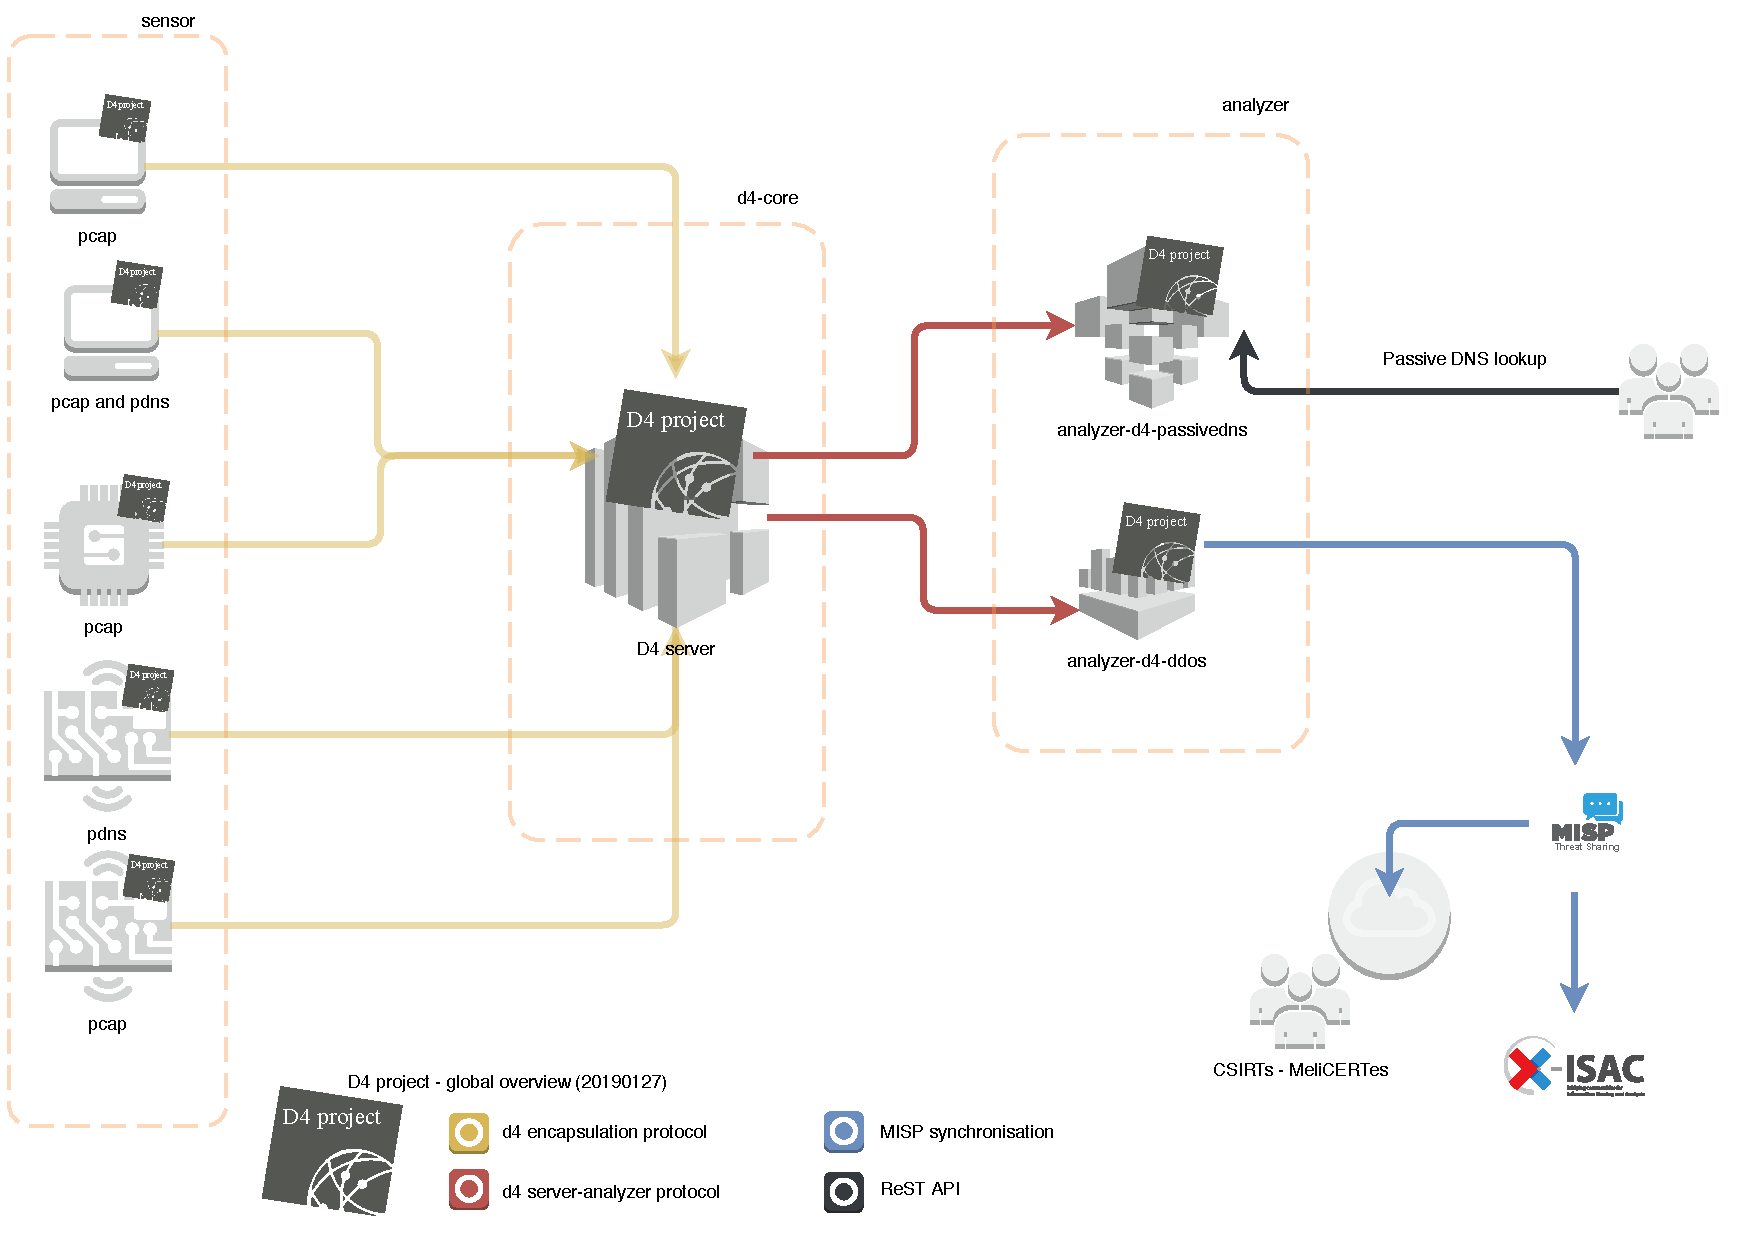
\includegraphics[scale=0.38]{d4-overview.pdf}
\end{frame}

\begin{frame}
\frametitle{Get in touch if you want to join/support the project, host a passive dns sensor or contribute}
\begin{itemize}
\item Collaboration can include research partnership, sharing of collected streams or improving the software.
\item Contact: info@circl.lu
\item \url{https://github.com/D4-Project} -  \url{https://twitter.com/d4_project}
\end{itemize}
\end{frame}


\end{document}
